\documentclass[12pt,a4paper]{article}
\usepackage[utf8]{inputenc}
\usepackage[T1]{fontenc}
\usepackage[english]{babel}
\usepackage{lmodern}
\usepackage{csquotes}
\usepackage{amsmath}
\usepackage{amsfonts}
\usepackage{amssymb}
\usepackage{physics}
\usepackage{geometry}
\usepackage{tocloft}
\usepackage{xcolor}
\usepackage{graphicx,tikz,pgfplots}
\pgfplotsset{compat=1.18}
\usepackage{booktabs}
\usepackage{array}
\usepackage{tabularx}
\usepackage{braket}
\usepackage{siunitx}
\usepackage{amsthm}
\usepackage[colorlinks=true, linkcolor=blue, citecolor=blue, urlcolor=blue]{hyperref}
\usepackage{cleveref}
\usepackage{fancyhdr} % Loaded last to avoid conflicts

\geometry{a4paper, margin=2.5cm}

\hypersetup{
	colorlinks=true,
	linkcolor=blue,
	filecolor=magenta,
	urlcolor=blue,
	pdftitle={Field Theory and Quantum Correlations: A New Perspective on Instantaneity},
	pdfauthor={Johann Pascher},
	pdfcreator={LaTeX}
}

\renewcommand{\cftsecfont}{\color{blue}}
\renewcommand{\cftsubsecfont}{\color{blue}}
\renewcommand{\cftsecpagefont}{\color{blue}}
\renewcommand{\cftsubsecpagefont}{\color{blue}}
\setlength{\cftsecindent}{1cm}
\setlength{\cftsubsecindent}{2cm}

\newcommand{\DhiggsT}{T(x) (\partial_\mu + igA_\mu)\Phi + \Phi \partial_\mu T(x)}
\newcommand{\Tfield}{T(x)}

\newtheorem{theorem}{Theorem}[section]
\newtheorem{proposition}[theorem]{Proposition}

\title{Field Theory and Quantum Correlations: \\ A New Perspective on Instantaneity}
\author{Johann Pascher}
\date{March 28, 2025}

\begin{document}
	
	\maketitle
	
	\begin{abstract}
		This work develops a new perspective on the phenomenon of quantum correlations and their apparent instantaneity. By introducing a fundamental field approach, it demonstrates how the nonlocal properties of quantum mechanics can be understood as a natural consequence of an underlying field structure. Particular attention is given to the role of the quantum background and the interpretation of modern Bell experiments. This perspective complements the time-mass duality theory, providing a consistent framework for understanding quantum phenomena within a comprehensive field concept.
	\end{abstract}
	
	\tableofcontents
	\newpage
	
	\section{Introduction}
	Modern quantum physics faces a fundamental challenge: The apparent instantaneity of quantum correlations seems to contradict our classical notions of locality and causality. Since the groundbreaking Bell experiments, particularly the loophole-free tests since 2015 \cite{Hensen2015}\relax, we know with certainty that the quantum world exhibits nonlocal properties. Yet, the question of the \textit{nature} of this nonlocality and its compatibility with relativity remains open.
	
	\subsection{A New Approach}
	This work develops an alternative perspective on the problem of quantum correlations by proposing a fundamental field approach. Instead of separate quantum fields, a unified fundamental field is postulated, in which particles appear as field nodes and quantum correlations as field properties \cite{Wilczek2008}\relax. This viewpoint allows the apparent `spooky action at a distance' to be understood as a natural consequence of the field structure.
	
	\subsection{Theoretical Foundations}
	\begin{theorem}[Field Concept]
		The proposed approach is based on three core concepts:
		\begin{itemize}
			\item The vacuum as an active quantum background with defined properties (\(\varepsilon_0\), \(\mu_0\)).
			\item Particles as stable nodes or excitation patterns in the fundamental field.
			\item Quantum correlations as inherent properties of field coherence.
		\end{itemize}
	\end{theorem}
	These concepts are directly linked to the time-mass duality theory \cite{Pascher2024}\relax, where the intrinsic time field \(T(x) = \hbar/mc^2\) is considered a fundamental quantity. The properties of the quantum background determine both the system's time evolution and the structure of the field nodes perceived as matter.
	
	\subsection{Experimental Evidence}
	The theory is supported by modern experiments, notably:
	\begin{itemize}
		\item The Vienna experiments of 2015, which closed all classical loopholes \cite{Giustina2015}\relax.
		\item The `Big Bell Test' of 2018 with its unique methodology \cite{BigBellTest2018}\relax.
		\item Various analogies to classical field phenomena.
	\end{itemize}
	
	\subsection{Mathematical Framework}
	The fundamental field equation can be written as:
	\begin{equation}
		\Box \Psi + V(\Psi) = 0
	\end{equation}
	where \(\Box = \frac{\partial^2}{\partial t^2} - c^2 \nabla^2\) is the d'Alembert operator and \(V(\Psi)\) is a potential term ensuring the stability of field nodes. In conjunction with time-mass duality, this equation can be reformulated as:
	\begin{equation}
		\left(\frac{\partial^2}{\partial(t/T(x))^2} - \nabla^2 + m_H^2\right) h_T(x) = 0
	\end{equation}
	for scalar fields like the Higgs field, and for fermions according to the modified Dirac equation:
	\begin{equation}
		\left(i\gamma^0\frac{\partial}{\partial(t/T(x))} + i\gamma^i\partial_i - m_f\right) \psi_T(x) = 0
	\end{equation}
	where the modified time derivative \(\partial_{t/T} = \frac{\partial}{\partial(t/T(x))} = T(x)\frac{\partial}{\partial t}\) is used \cite{Pascher2024}\relax. This leads to a modified dispersion relation:
	\begin{equation}
		\omega_T^2 = \mathbf{k}^2 + \frac{m_H^2 c^4}{\hbar^2} \cdot T(x)^2
	\end{equation}
	
	\section{The Vacuum as Quantum Background}
	The vacuum is not merely 'nothing' but an active quantum background with defined physical properties \cite{Milonni1994}\relax.
	
	\subsection{Fundamental Vacuum Constants}
	The electric field constant (\(\varepsilon_0\)) and magnetic field constant (\(\mu_0\)) characterize the fundamental properties of the vacuum as a quantum background. They determine interactions in the electromagnetic field and are directly related to the speed of light:
	\begin{equation}
		c = \frac{1}{\sqrt{\varepsilon_0 \mu_0}}
	\end{equation}
	These constants are not just mathematical quantities but expressions of the physical structure of the quantum background \cite{Aitchison2004}\relax. In the time-mass duality theory, they directly influence the intrinsic time field \(T(x)\) and thus the energy scale of field nodes \cite{Pascher2024}\relax.
	
	\subsection{The Vacuum as Field Carrier}
	The quantum background acts as a carrier medium for the electromagnetic field and all other fundamental fields. This perspective enables:
	\begin{itemize}
		\item Explaining wave propagation in 'empty' space.
		\item Understanding nonlocal correlations as inherent field properties.
		\item Overcoming the limits of classical particle concepts.
	\end{itemize}
	The homogeneity of the vacuum and its properties (\(\varepsilon_0\), \(\mu_0\)) is crucial for the constancy of the speed of light and thus the validity of special relativity \cite{Weinberg1995}\relax.
	
	\section{Quantum Correlations in the Field Model}
	\subsection{Polarization and Entanglement}
	The polarization of a photon can be described as a superposition of horizontal (H) and vertical (V) polarization \cite{Fox2006}\relax:
	\begin{equation}
		|\psi\rangle = \alpha |H\rangle + \beta e^{i\phi} |V\rangle
	\end{equation}
	For entangled photon pairs, a joint state arises such as:
	\begin{equation}
		|\psi\rangle = \frac{1}{\sqrt{2}} (|H\rangle_A |H\rangle_B + |V\rangle_A |V\rangle_B)
	\end{equation}
	In the field model, these states are not considered isolated particle properties but coherent field patterns extending across space \cite{Zeilinger2010}\relax. The correlation between measurements on particles A and B is an inherent property of this field pattern, not the result of instantaneous 'communication' between the particles.
	
	\subsection{Bell Inequalities and Local Realism}
	Bell inequalities and their experimental violation demonstrate the limits of local realistic theories \cite{Bell1964}\relax. In the field model, this can be understood as:
	\begin{equation}
		|E(a,b) - E(a,c)| \leq 1 + E(b,c)
	\end{equation}
	The experimentally observed violation of this inequality (for certain angles a, b, c) shows that the quantum world cannot be described by local hidden variables \cite{Aspect1982}\relax. The field model provides a natural explanation: The fundamental field is inherently nonlocal, as it spans the entire space.
	
	\subsection{The Vienna Experiment of 2015}
	The experiment by Anton Zeilinger's group in Vienna in 2015 was one of the first truly loophole-free tests of Bell's theorem \cite{Giustina2015}\relax. It combined:
	\begin{itemize}
		\item Very high detection efficiency (>97\% using SNSPDs).
		\item Sufficient spatial separation of measurements.
		\item Fast, independent quantum random number generators.
	\end{itemize}
	The observed violation of the Bell inequality with a statistical significance of 11.5 standard deviations confirms the nonlocality of the quantum world. In the field model, this nonlocality is a natural property of the fundamental field and its coherent structure \cite{Zeilinger2010}\relax.
	
	\subsection{The "Big Bell Test" of 2018}
	The "Big Bell Test" utilized decisions from over 100,000 people worldwide to control measurement settings in 13 different labs \cite{BigBellTest2018}\relax. This human component addressed the freedom-of-choice loophole in a novel way. The results showed a violation of Bell inequalities with statistical significances up to 70 standard deviations.
	These experiments confirm the nonlocal nature of the quantum world, which can be understood in the field model as an expression of the coherent field structure.
	
	\section{Field Theory and Instantaneity}
	\subsection{Sound Waves as an Analogy}
	Sound waves provide a useful analogy for understanding the field concept \cite{Bohm1980}\relax:
	\begin{itemize}
		\item Sound exists as a pressure wave permeating the entire space.
		\item A microphone measures the vibration locally, but the wave itself is globally present.
		\item The simultaneity of measurements at different microphones arises from the coherent structure of the sound wave.
	\end{itemize}
	In the field model, entangled particles are like nodes in a global quantum field. The correlations between them are not 'action at a distance' but inherent properties of the field, sampled locally during measurement. The Higgs field plays a special role as a universal medium that not only imparts mass but also determines the intrinsic timescale of all particles, as described in the time-mass duality theory \cite{Pascher2024}\relax.
	
	\subsection{Why This Analogy Matters}
	\subsubsection{Resolution of the Paradox}
	Nonlocality appears paradoxical only when particles are viewed as separate objects. In the field model, they are parts of a whole – like sound wave points in a room \cite{Bohm1980}\relax.
	
	\subsubsection{Reality of the Field}
	The quantum field is not an abstraction but the fundamental entity \cite{Weinberg1995}\relax. Its properties (coherence, nonlocality) are as real as those of a sound wave.
	
	\subsubsection{Experimental Consequence}
	When Alice and Bob measure entangled photons, they are essentially 'listening' to two microphones sampling the same sound wave. The correlations are already contained in the field, not generated at the moment of measurement \cite{Zeilinger2010}\relax.
	
	In the context of the time-mass duality theory, these correlations gain an additional temporal dimension: The intrinsic time field \(\Tfield = \hbar/mc^2\) determines the timescale of field correlations, providing a natural explanation for the observed coherence times and their mass dependence \cite{Pascher2024}\relax. The modified Higgs-Yukawa coupling
	\begin{equation}
		\mathcal{L}_{\text{Yukawa-T}} = -y_f \bar{\psi}_L \Phi \psi_R + \text{h.c.}
	\end{equation}
	defines not only the mass of particles but also their intrinsic timescale according to
	\begin{equation}
		\Tfield = \frac{\hbar}{m(x) c^2} = \frac{\hbar \sqrt{2}}{y_f v c^2}
	\end{equation}
	This relationship establishes a fundamental link between the Higgs mechanism and quantum coherence.
	
	\section{Field Equations in Dual Formulation}
	\subsection{Modified Quantum Mechanics with Variable Mass}
	In contrast to the conventional Schrödinger equation:
	\begin{equation}
		i\hbar \frac{\partial}{\partial t}\Psi(x,t) = \hat{H}\Psi(x,t)
	\end{equation}
	where time (\(t\)) is treated as an external, classical parameter and mass is constant, the time-mass duality introduces a fundamental modification:
	\begin{equation}
		i\hbar \frac{\partial}{\partial (t/\Tfield)}\Psi = \hat{H}\Psi
	\end{equation}
	This modified equation uses the intrinsic time field \(\Tfield = \hbar/mc^2\) and accounts for the fact that time evolution is no longer uniform for all objects but depends on their mass. For systems with variable mass, this can be rewritten as:
	\begin{equation}
		i\hbar \frac{\partial}{\partial t}\Psi(x,t) = \hat{H}(m(t))\Psi(x,t)
	\end{equation}
	For multi-particle systems with different masses, as encountered in entangled systems, the modified equation takes the form:
	\begin{equation}
		i (m_1 + m_2) c^2 \frac{\partial}{\partial t} \Psi(x_1, x_2, t) = \hat{H} \Psi(x_1, x_2, t)
	\end{equation}
	This extension has profound implications for our understanding of quantum correlations and the apparent instantaneity in entangled states \cite{Pascher2024}\relax.
	
	\subsection{Klein-Gordon Equation and Higgs Field}
	The standard Klein-Gordon equation for the Higgs boson is:
	\begin{equation}
		(\Box + m_H^2) h(x) = 0
	\end{equation}
	In the time-mass duality framework, it becomes:
	\begin{equation}
		\left(\frac{\partial^2}{\partial(t/\Tfield)^2} - \nabla^2 + m_H^2\right) h_T(x) = 0
	\end{equation}
	This leads to a modified dispersion relation:
	\begin{equation}
		\omega_T^2 = \mathbf{k}^2 + \frac{m_H^2 c^4}{\hbar^2} \cdot T(x)^2
	\end{equation}
	
	\subsection{Dirac Equation for Fermions}
	The Dirac equation for fermions in the standard model is:
	\begin{equation}
		(i\gamma^\mu\partial_\mu - m_f) \psi(x) = 0
	\end{equation}
	In the time-mass duality framework, it becomes:
	\begin{equation}
		\left(i\gamma^0\frac{\partial}{\partial(t/\Tfield)} + i\gamma^i\partial_i - m_f\right) \psi_T(x) = 0
	\end{equation}
	
	\subsection{Variable Mass as a Hidden Variable}
	A particularly fascinating consequence of this perspective is that variable mass could serve as a fundamental hidden variable, potentially explaining the apparent indeterminism of quantum mechanics. Unlike classical hidden variable theories, largely ruled out by Bell experiments, the variable mass in time-mass duality is a fundamental, physically grounded quantity.
	The modified Lagrangian density formalizing this approach is:
	\begin{equation}
		\mathcal{L}_\text{total} = \mathcal{L}_\text{Standard} + \mathcal{L}_\text{intrinsic}
	\end{equation}
	where the additional term accounts for the intrinsic time field:
	\begin{equation}
		\mathcal{L}_\text{intrinsic} = \bar{\psi}\left(i\hbar\gamma^0 \frac{\partial}{\partial (t/\Tfield)} - i\hbar\gamma^0 \frac{\partial}{\partial t}\right)\psi
	\end{equation}
	This extension could pave the way for a deterministic quantum theory, affirming Einstein’s intuition that 'God does not play dice' \cite{Pascher2024}\relax.
	
	\section{Field Theory and Locality}
	\subsection{Local-Realistic Models and Hidden Variables}
	In a local-realistic theory, measurement outcomes would need to be determined by local hidden variables \(\lambda\) \cite{Bell1964}\relax. The correlation function would then be:
	\begin{equation}
		E(a,b) = \int A(a,\lambda)B(b,\lambda)\rho(\lambda)d\lambda
	\end{equation}
	However, Bell experiments show that this assumption cannot explain the observed correlations \cite{Aspect1982}\relax.
	
	\subsection{The Wave Field Model as an Alternative}
	The wave field model offers an alternative that can explain quantum correlations without violating locality \cite{Bohm1980}\relax:
	\begin{itemize}
		\item The entangled system is considered a unified, coherent field.
		\item Measurements at different locations are local samplings of this global field.
		\item Correlations are inherent properties of the field, not the result of instantaneous communication.
	\end{itemize}
	This model is consistent with the time-mass duality theory, as both approaches view the fundamental field and its inherent correlations as the primary reality \cite{Pascher2024}\relax. The Higgs field can be understood in this context as a universal medium, described by the modified Lagrangian density
	\begin{equation}
		\mathcal{L}_{\text{Higgs-T}} = (\DhiggsT)^\dagger (\DhiggsT) - \lambda(|\Phi|^2 - v^2)^2
	\end{equation}
	The modified covariant derivative
	\begin{equation}
		\DhiggsT = T(x) (\partial_\mu + igA_\mu)\Phi + \Phi \partial_\mu T(x)
	\end{equation}
	incorporates the temporal modification with respect to the intrinsic time field, making the Higgs field a central mediator between space, time, and mass.
	
	\subsection{Field Coherence and Nonlocality}
	Nonlocality in the field model is not interpreted as 'spooky action at a distance' but as an expression of the coherence of an extended system \cite{Zeilinger2010}\relax:
	\begin{itemize}
		\item The entangled wave field directly connects the measurement locations through its coherent properties.
		\item The apparent 'communication' is not a transfer of information but the result of a shared field state.
	\end{itemize}
	The time-mass duality theory complements this picture by identifying the intrinsic time field \(\Tfield\) as the characteristic timescale of field correlations. This explains the observed coherence times and their dependence on mass \cite{Pascher2024}\relax. For quantum systems of different masses, the coherence times \(\tau_1\) and \(\tau_2\) of two otherwise identical quantum systems with masses \(m_1\) and \(m_2\) should follow the ratio:
	\begin{equation}
		\frac{\tau_1}{\tau_2} = \frac{m_2}{m_1}
	\end{equation}
	This prediction could be tested through precision experiments with entangled particles of different masses, establishing a direct link between classical nonlocality and the mass-dependent timescale of the quantum system.
	
	\section{Field Theory and Relativity}
	\subsection{The Wave Field Model and Relativity}
	The wave field model can be reconciled with relativity \cite{Maudlin2011}\relax:
	\begin{itemize}
		\item No true information transfer: Correlations between entangled particles do not arise from signal transmission.
		\item Locality of measurement outcomes: Each measurement value is determined locally, even if the results are globally correlated.
		\item Extended field: The field spans all space but is constrained by the light cone structure of spacetime.
	\end{itemize}
	
	\subsection{Relativistic Quantum Field Theory and Variable Mass}
	The wave field model is also compatible with relativistic quantum field theory \cite{Weinberg1995}\relax:
	\begin{itemize}
		\item Entanglement in spacetime: Quantum correlations are fully describable in relativistic quantum field theory.
		\item No absolute reference time: Relativity requires no preferred time coordinate, and the wave field model does not assume one.
	\end{itemize}
	These considerations indicate that the concepts of locality and realism must be reinterpreted without violating fundamental principles like relativity. The time-mass duality theory offers a promising approach by bridging two complementary perspectives:
	\begin{itemize}
		\item The standard model with constant mass and time dilation (the usual relativistic framework).
		\item The complementary model with absolute time and variable mass.
	\end{itemize}
	This duality enables a new interpretation of relativistic phenomena and quantum mechanical processes, with the Higgs field acting as a mediator between the two descriptions. The modified dispersion relation
	\begin{equation}
		\omega_T^2 = \mathbf{k}^2 + \frac{m_H^2 c^4}{\hbar^2} \cdot T(x)^2
	\end{equation}
	demonstrates how this duality manifests in wave propagation \cite{Pascher2024}\relax.
	
	\subsection{The Paradox of Instantaneity and the Role of Variable Mass}
	The apparent instantaneity of quantum correlations remains one of the most persistent paradoxes in quantum mechanics. The notion that measurements on entangled particles, regardless of their spatial separation, yield instantaneously correlated results seems to contradict relativity, which prohibits superluminal information transfer.
	The time-mass duality theory provides an elegant solution to this paradox:
	\begin{itemize}
		\item In conventional views, quantum correlations appear instantaneous because we treat time as a universal, constant parameter.
		\item Within the time-mass duality framework with variable mass, it becomes evident that the mass-dependent intrinsic time field \(\Tfield = \hbar/mc^2\) represents a more fundamental timescale than external lab time.
		\item Correlations do not occur instantaneously in the system's intrinsic time but follow a dynamic described by the modified Schrödinger equation
		\begin{equation}
			i\hbar \frac{\partial}{\partial (t/\Tfield)}\Psi = \hat{H}\Psi
		\end{equation}
	\end{itemize}
	This reformulation resolves the paradox naturally: What appears as instantaneous action in lab time is actually a process unfolding in the intrinsic time of the quantum system, with variable mass acting as a hidden variable \cite{Pascher2024}\relax. The modified Lagrangian density
	\begin{equation}
		\mathcal{L}_\text{intrinsic} = \bar{\psi}\left(i\hbar\gamma^0 \frac{\partial}{\partial (t/\Tfield)} - i\hbar\gamma^0 \frac{\partial}{\partial t}\right)\psi
	\end{equation}
	formally captures the discrepancy between time evolution in absolute time and mass-dependent intrinsic time.
	
	\begin{figure}[h]
		\centering
		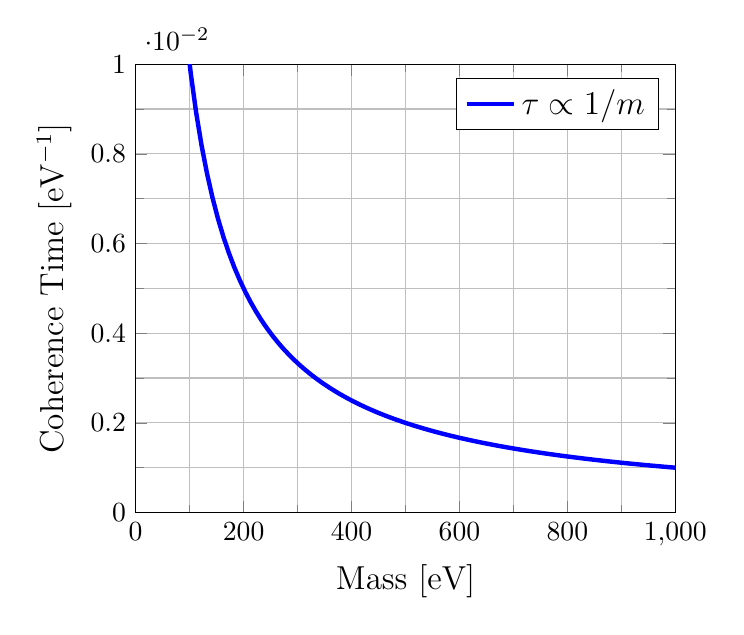
\begin{tikzpicture}
			\begin{axis}[
				xlabel={Mass [eV]},
				ylabel={Coherence Time [eV\(^{-1}\)]},
				xlabel style={font=\large},
				ylabel style={font=\large},
				tick label style={font=\normalsize},
				xmin=0, xmax=1000,
				ymin=0, ymax=0.01,
				legend pos=north east,
				legend style={font=\large},
				grid=both,
				minor tick num=1
				]
				\addplot[blue, ultra thick, domain=1:1000, samples=100] {1/x};
				\legend{\(\tau \propto 1/m\)}
			\end{axis}
		\end{tikzpicture}
		\caption{Mass-dependent coherence time in the field model.}
	\end{figure}
	
	\bibliographystyle{plainnat}
	\begin{thebibliography}{99}
		\bibitem{Aitchison2004} Aitchison, I. J. R. (2004). \textit{An Informal Introduction to Gauge Field Theories}. Cambridge University Press.
		\bibitem{Aspect1982} Aspect, A., Grangier, P., \& Roger, G. (1982). \textit{Experimental Realization of Einstein-Podolsky-Rosen-Bohm Gedankenexperiment: A New Violation of Bell's Inequalities}. Physical Review Letters, 49(2), 91-94.
		\bibitem{Bell1964} Bell, J. S. (1964). \textit{On the Einstein Podolsky Rosen Paradox}. Physics Physique Fizika, 1(3), 195-200.
		\bibitem{BigBellTest2018} BIG Bell Test Collaboration. (2018). \textit{Challenging Local Realism with Human Choices}. Nature, 557(7704), 212-216.
		\bibitem{Bohm1980} Bohm, D. (1980). \textit{Wholeness and the Implicate Order}. Routledge.
		\bibitem{Feynman1965} Feynman, R. P. (1965). \textit{The Character of Physical Law}. MIT Press.
		\bibitem{Fox2006} Fox, M. (2006). \textit{Quantum Optics: An Introduction}. Oxford University Press.
		\bibitem{Giustina2015} Giustina, M., et al. (2015). \textit{Significant-Loophole-Free Test of Bell's Theorem with Entangled Photons}. Physical Review Letters, 115(25), 250401.
		\bibitem{Handsteiner2017} Handsteiner, J., et al. (2017). \textit{Cosmic Bell Test: Measurement Settings from Milky Way Stars}. Physical Review Letters, 118(6), 060401.
		\bibitem{Hensen2015} Hensen, B., et al. (2015). \textit{Loophole-Free Bell Inequality Violation Using Electron Spins Separated by 1.3 Kilometres}. Nature, 526(7575), 682-686.
		\bibitem{Jozsa2000} Jozsa, R., et al. (2000). \textit{Quantum Clock Synchronization Based on Shared Prior Entanglement}. Physical Review Letters, 85(9), 2010-2013.
		\bibitem{Maudlin2011} Maudlin, T. (2011). \textit{Quantum Non-Locality and Relativity: Metaphysical Intimations of Modern Physics}. John Wiley \& Sons.
		\bibitem{Milonni1994} Milonni, P. W. (1994). \textit{The Quantum Vacuum: An Introduction to Quantum Electrodynamics}. Academic Press.
		\bibitem{Pascher2024a} Pascher, J. (2024). \textit{Time-Mass Duality: A New Approach to Unifying Fundamental Forces}.
		\bibitem{Pascher2024b} Pascher, J. (2024). \textit{Mathematical Formulation of the Higgs Mechanism in Time-Mass Duality}.
		\bibitem{Pascher2024c} Pascher, J. (2024). \textit{The Necessity of Extending Standard Quantum Mechanics and Quantum Field Theory}.
		\bibitem{Pascher2024} Pascher, J. (2024). \textit{Essential Mathematical Formalisms of the Time-Mass Duality Theory with Lagrangian Densities}. March 29, 2025.
		\bibitem{Schlosshauer2013} Schlosshauer, M. (2013). \textit{Elegance and Enigma: The Quantum Interviews}. Springer.
		\bibitem{Shimony2017} Shimony, A. (2017). \textit{Bell's Theorem}. In The Stanford Encyclopedia of Philosophy (Fall 2017 Edition), Edward N. Zalta (ed.).
		\bibitem{Wallace2012} Wallace, D. (2012). \textit{The Emergent Multiverse: Quantum Theory According to the Everett Interpretation}. Oxford University Press.
		\bibitem{Weinberg1995} Weinberg, S. (1995). \textit{The Quantum Theory of Fields, Volume 1: Foundations}. Cambridge University Press.
		\bibitem{Wilczek2008} Wilczek, F. (2008). \textit{The Lightness of Being: Mass, Ether, and the Unification of Forces}. Basic Books.
		\bibitem{Yin2017} Yin, J., et al. (2017). \textit{Satellite-Based Entanglement Distribution Over 1200 Kilometers}. Science, 356(6343), 1140-1144.
		\bibitem{Zeilinger2010} Zeilinger, A. (2010). \textit{Dance of the Photons: From Einstein to Quantum Teleportation}. Farrar, Straus and Giroux.
	\end{thebibliography}
	
\end{document}